\subsection*{Problema 48}

\textbf{Enunciado:}
Calcular la siguiente integral indefinida:
\begin{align*}
\int \frac{x}{\sqrt{x^2 + 2x + 2}} \, dx
\end{align*}

\textbf{Solución:}

Siguiendo la indicación, el objetivo es expresar el numerador en función de la derivada de la cantidad subradical. Sea $u = x^2 + 2x + 2$, su derivada es $du = (2x + 2) \, dx$. 

Manipulamos algebraicamente el numerador de la integral para que aparezca dicha derivada:
\begin{align*}
x &= \dfrac{1}{2}(2x) \\
&= \dfrac{1}{2}(2x + 2 - 2) \\
&= \dfrac{1}{2}(2x + 2) - 1
\end{align*}

Sustituimos esta expresión en el numerador de la integral original:
\begin{align*}
\int &\dfrac{x}{\sqrt{x^2 + 2x + 2}} \, dx = \\
&\int \dfrac{\frac{1}{2}(2x + 2) - 1}{\sqrt{x^2 + 2x + 2}} \, dx
\end{align*}

Separamos la integral en dos partes distintas:
\begin{align*}
&= \dfrac{1}{2} \int \dfrac{2x + 2}{\sqrt{x^2 + 2x + 2}} \, dx \\
&\quad - \int \dfrac{1}{\sqrt{x^2 + 2x + 2}} \, dx
\end{align*}

Para la primera integral, usamos sustitución directa con $u = x^2 + 2x + 2$ y $du = (2x + 2) \, dx$:
\begin{align*}
I_1 &= \dfrac{1}{2} \int u^{-1/2} \, du \\
&= \dfrac{1}{2} \left( 2u^{1/2} \right) = \sqrt{u} \\
&= \sqrt{x^2 + 2x + 2}
\end{align*}

Para la segunda integral, completamos el trinomio cuadrado perfecto en el denominador:
\begin{align*}
x^2 + 2x + 2 &= (x^2 + 2x + 1) + 1 \\
&= (x + 1)^2 + 1
\end{align*}

Sustituimos esto en la segunda integral $I_2$:
\begin{align*}
I_2 &= \int \dfrac{1}{\sqrt{(x + 1)^2 + 1}} \, dx
\end{align*}

Esta integral se resuelve mediante la fórmula estándar de sustitución trigonométrica o integración directa con funciones hiperbólicas/logarítmicas:
\begin{align*}
I_2 &= \ln\left| (x + 1) + \sqrt{(x + 1)^2 + 1} \right| \\
&= \ln\left| x + 1 + \sqrt{x^2 + 2x + 2} \right|
\end{align*}

Finalmente, combinamos ambos resultados y añadimos la constante de integración $C$:
\begin{align*}
\int &\dfrac{x}{\sqrt{x^2 + 2x + 2}} \, dx = \sqrt{x^2 + 2x + 2} \\
&\quad - \ln\left| x + 1 + \sqrt{x^2 + 2x + 2} \right| + C
\end{align*}

\begin{figure}[H]
	\centering
	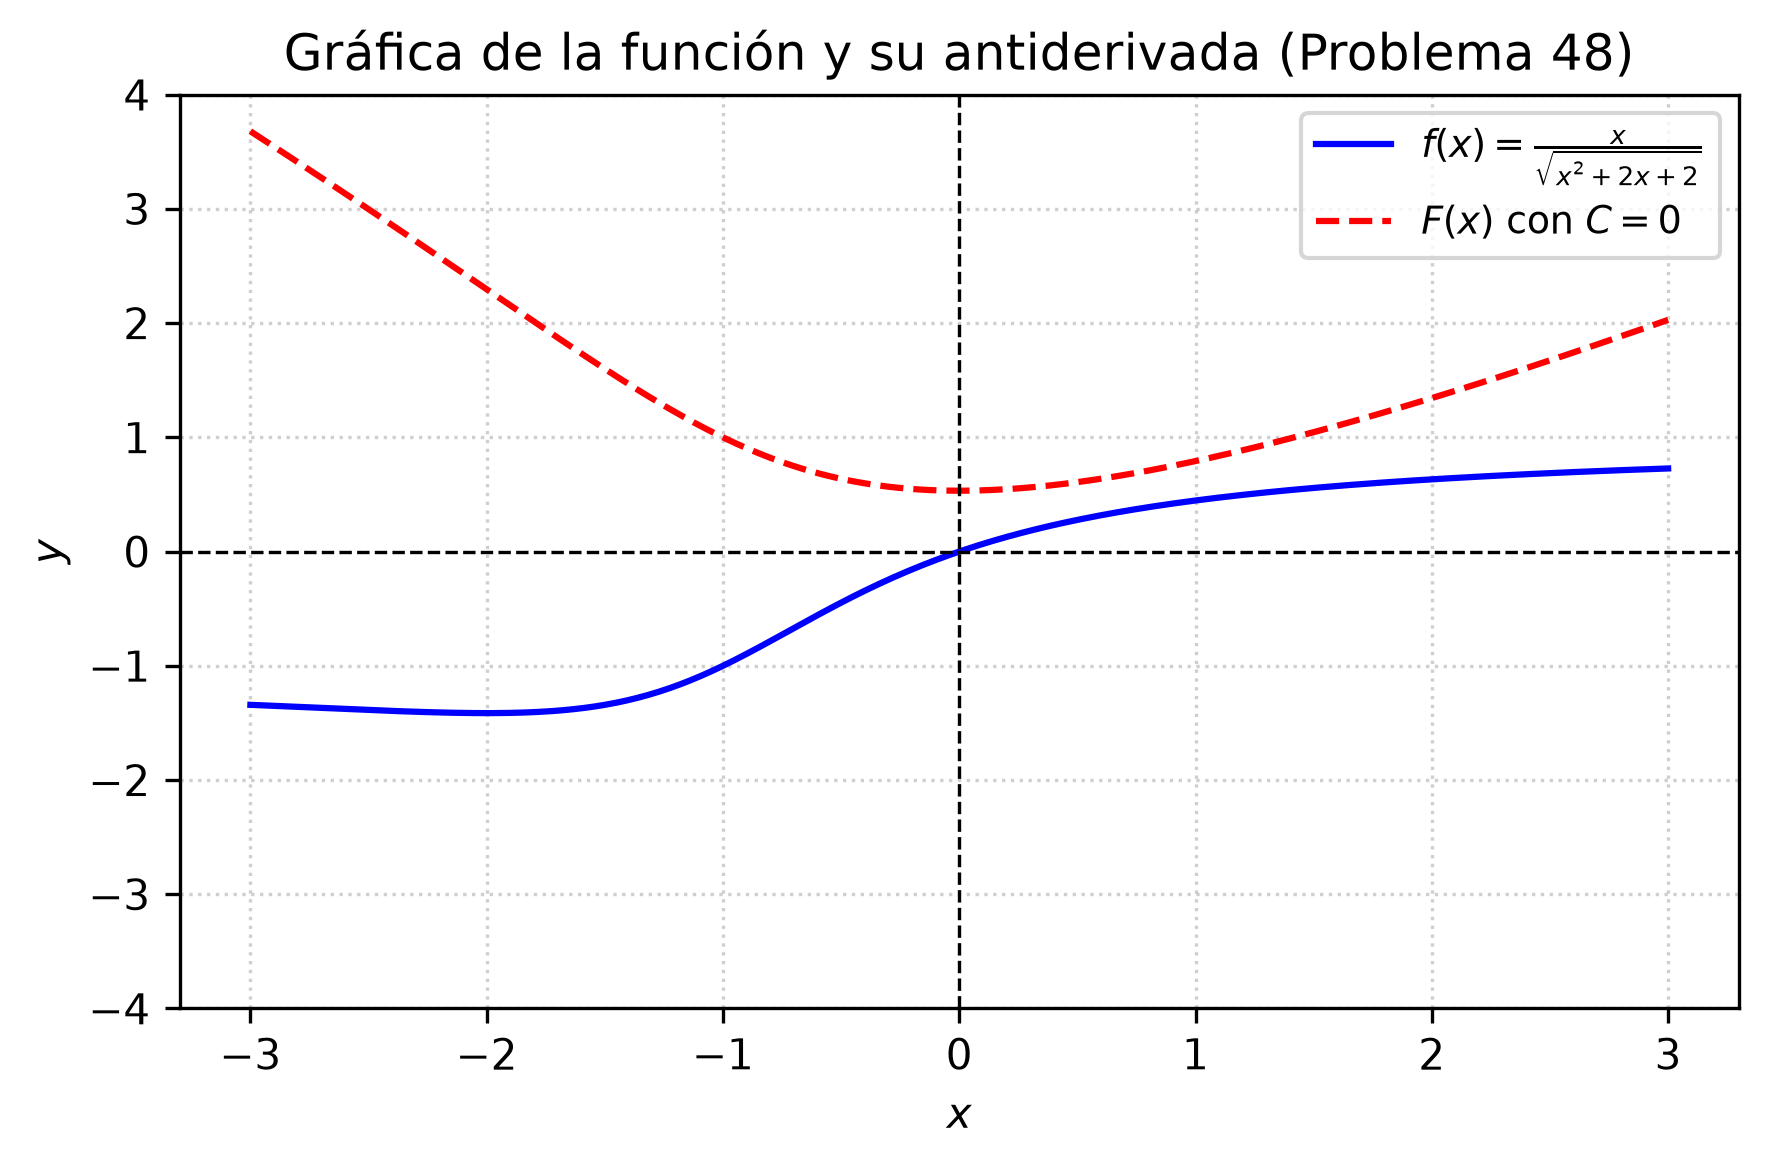
\includegraphics[width=\columnwidth]{semana_05/graficas/SEM05_P48_grafica.png}
	\caption{Representación gráfica de $f(x)$ y su antiderivada $F(x)$ evaluada para la constante de integración $C = 0$ (Problema 48).}
	\label{fig:problema48}
\end{figure}
